\documentclass{article}
\usepackage{pgf,tikz}
\usepackage{mathrsfs}
\usetikzlibrary{arrows}
\pagestyle{empty}

%\usepackage[active,pdftex,tightpage]{preview}


%\PreviewEnvironment{tikzpicture}


\definecolor{ffqqqq}{rgb}{1.,0.,0.}
\definecolor{uuuuuu}{rgb}{0.266,0.266,0.266}

\begin{document}

% As figuras do ``Para o professor'' estão entre as demais.


%Enunciado

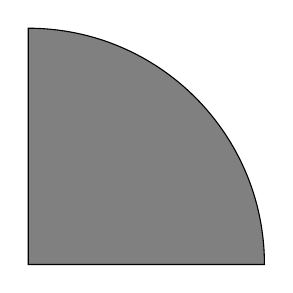
\begin{tikzpicture}
\draw [fill=gray] (0,0) arc (0:90:3) -- (-3,0) -- cycle;
\end{tikzpicture}
\vspace{1 cm}


\begin{tikzpicture}
\draw [fill=gray] (0,0) rectangle (3,3);
\end{tikzpicture}
\vspace{1 cm}

\begin{tikzpicture}
\draw  (0,0) -- (3,3);
\end{tikzpicture}
\vspace{1 cm}

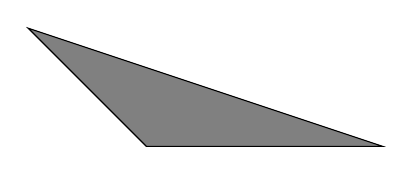
\begin{tikzpicture}
\draw [fill=gray] (0,0) -- (3,0) -- (-1.5,1.5) -- cycle;
\end{tikzpicture}
\vspace{1 cm}

% Respostas

% arcos de círculos 

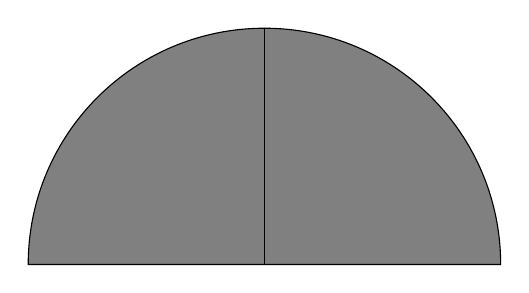
\begin{tikzpicture}%[line cap=round,line join=round,>=triangle 45,x=1.0cm,y=1.0cm]
\draw [fill=gray] (0,0) arc (0:180:3) -- (0,0) -- cycle;
\draw (-3,0) -- (-3,3);
\end{tikzpicture}


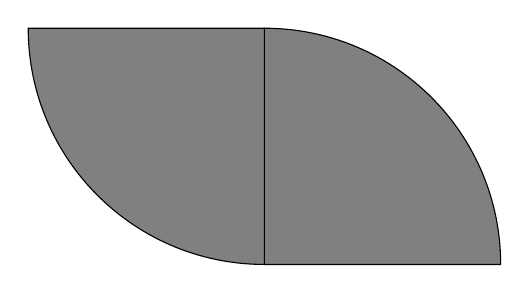
\begin{tikzpicture}%[line cap=round,line join=round,>=triangle 45,x=1.0cm,y=1.0cm]
\draw [fill=gray] (0,0) arc (0:90:3) -- (-3,0) -- cycle;
\draw [fill=gray] (-3,0) arc (270:180:3) -- (-3,3) -- cycle;
\end{tikzpicture}

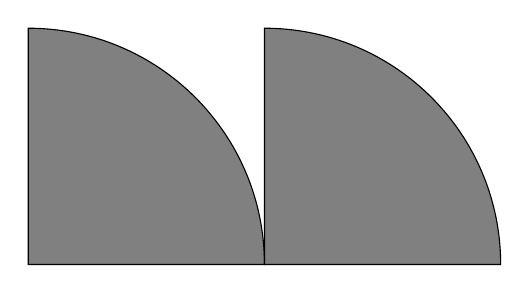
\begin{tikzpicture}%[line cap=round,line join=round,>=triangle 45,x=1.0cm,y=1.0cm]
\draw [fill=gray] (0,0) arc (0:90:3) -- (-3,0) -- cycle;
\draw [fill=gray] (3,0) arc (0:90:3) -- (0,0) -- cycle;
\end{tikzpicture}

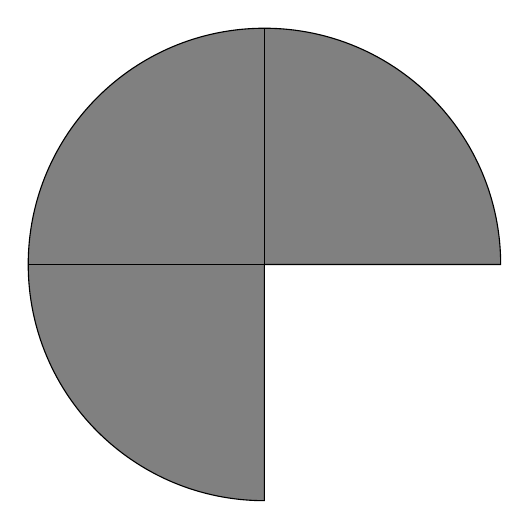
\begin{tikzpicture}%[line cap=round,line join=round,>=triangle 45,x=1.0cm,y=1.0cm]
\draw [fill=gray] (0,0) arc (0:270:3) -- (-3,0) -- cycle;
\draw (-3,0) -- (-6,0);
\draw (-3,0) -- (-3,3);
\end{tikzpicture}


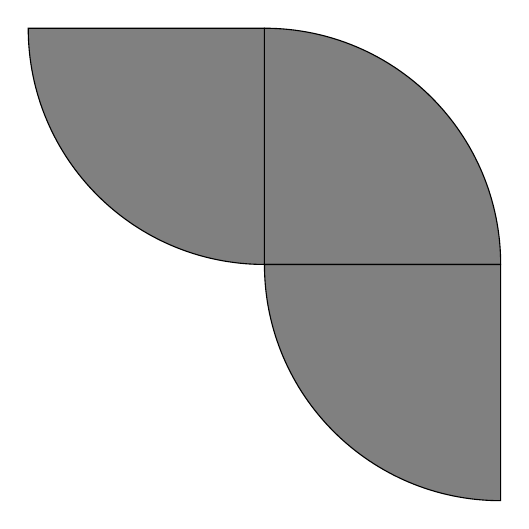
\begin{tikzpicture}%[line cap=round,line join=round,>=triangle 45,x=1.0cm,y=1.0cm]
\draw [fill=gray] (0,0) arc (0:90:3) -- (-3,0) -- cycle;
\draw [fill=gray] (-3,0) arc (270:180:3) -- (-3,3) -- cycle;
\draw [fill=gray] (-3,0) arc (180:270:3) -- (0,0) -- cycle;
\end{tikzpicture}

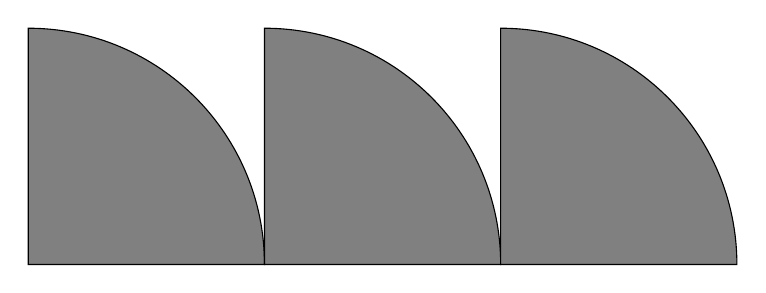
\begin{tikzpicture}%[line cap=round,line join=round,>=triangle 45,x=1.0cm,y=1.0cm]
\draw [fill=gray] (0,0) arc (0:90:3) -- (-3,0) -- cycle;
\draw [fill=gray] (3,0) arc (0:90:3) -- (0,0) -- cycle;
\draw [fill=gray] (6,0) arc (0:90:3) -- (3,0) -- cycle;
\end{tikzpicture}

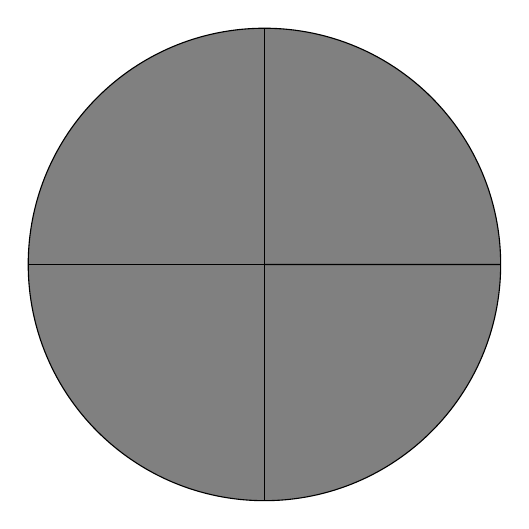
\begin{tikzpicture}%[line cap=round,line join=round,>=triangle 45,x=1.0cm,y=1.0cm]
\draw [fill=gray] (0,0) arc (0:360:3) -- (-3,0) -- cycle;
\draw (-3,0) -- (-6,0);
\draw (-3,0) -- (-3,3);
\draw (-3,0) -- (-3,-3);
\end{tikzpicture}

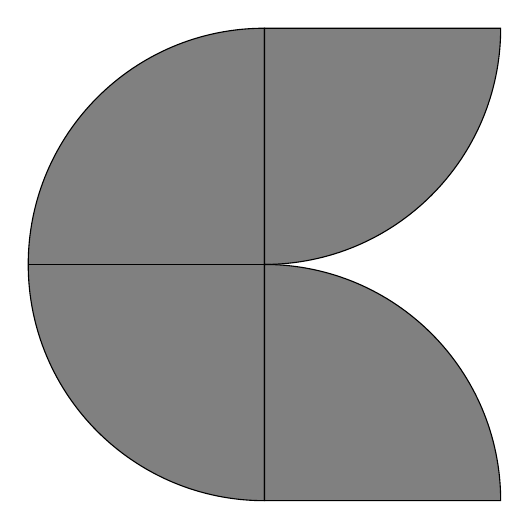
\begin{tikzpicture}%[line cap=round,line join=round,>=triangle 45,x=1.0cm,y=1.0cm]
\draw [fill=gray] (0,3) arc (90:270:3) -- (0,3) -- cycle;
 \draw [fill=gray] (3,3) arc (0:-90:3) -- (0,3) -- cycle;
 \draw [fill=gray] (0,0) arc (90:0:3) -- (0,-3) -- cycle;
 \draw  (0,0) -- (-3,0);
\end{tikzpicture}

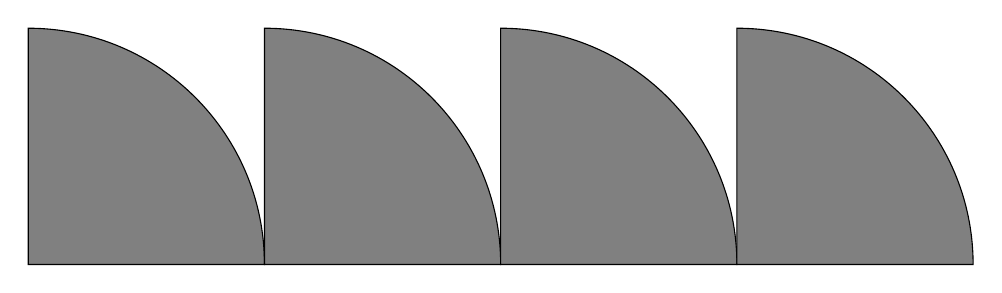
\begin{tikzpicture}%[line cap=round,line join=round,>=triangle 45,x=1.0cm,y=1.0cm]
\draw [fill=gray] (0,0) arc (0:90:3) -- (-3,0) -- cycle;
\draw [fill=gray] (3,0) arc (0:90:3) -- (0,0) -- cycle;
\draw [fill=gray] (6,0) arc (0:90:3) -- (3,0) -- cycle;
\draw [fill=gray] (9,0) arc (0:90:3) -- (6,0) -- cycle;
\end{tikzpicture}

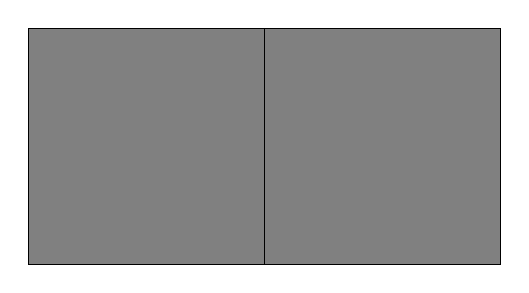
\begin{tikzpicture}%[line cap=round,line join=round,>=triangle 45,x=1.0cm,y=1.0cm]
\draw [fill=gray] (0,0) rectangle (3,3);
\draw [fill=gray] (3,0) rectangle (6,3);
\end{tikzpicture}

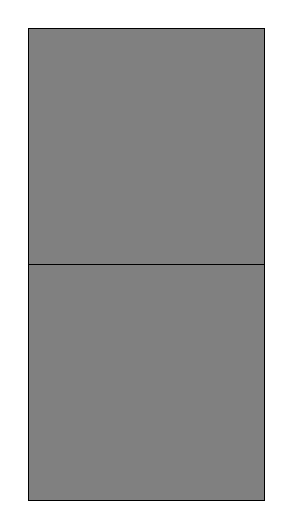
\begin{tikzpicture}%[line cap=round,line join=round,>=triangle 45,x=1.0cm,y=1.0cm]
\draw [fill=gray] (0,0) rectangle (3,3);
\draw [fill=gray] (0,3) rectangle (3,6);
\end{tikzpicture}

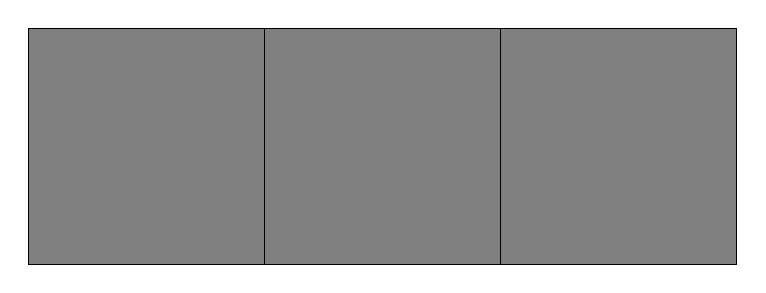
\begin{tikzpicture}%[line cap=round,line join=round,>=triangle 45,x=1.0cm,y=1.0cm]
\draw [fill=gray] (0,0) rectangle (3,3);
\draw [fill=gray] (3,0) rectangle (6,3);
\draw [fill=gray] (6,0) rectangle (9,3);
\end{tikzpicture}

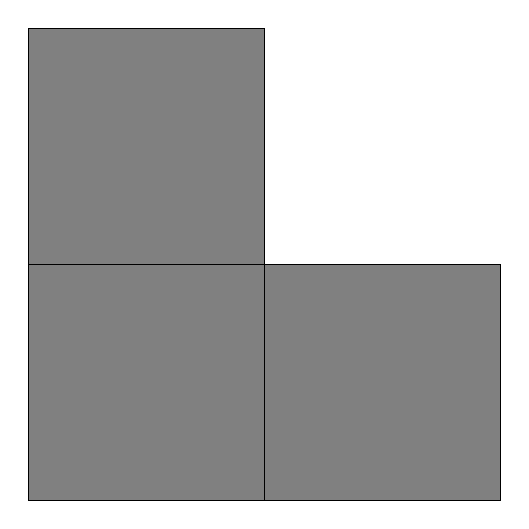
\begin{tikzpicture}%[line cap=round,line join=round,>=triangle 45,x=1.0cm,y=1.0cm]
\draw [fill=gray] (0,0) rectangle (3,3);
\draw [fill=gray] (0,3) rectangle (3,6);
\draw [fill=gray] (3,0) rectangle (6,3);
\end{tikzpicture}


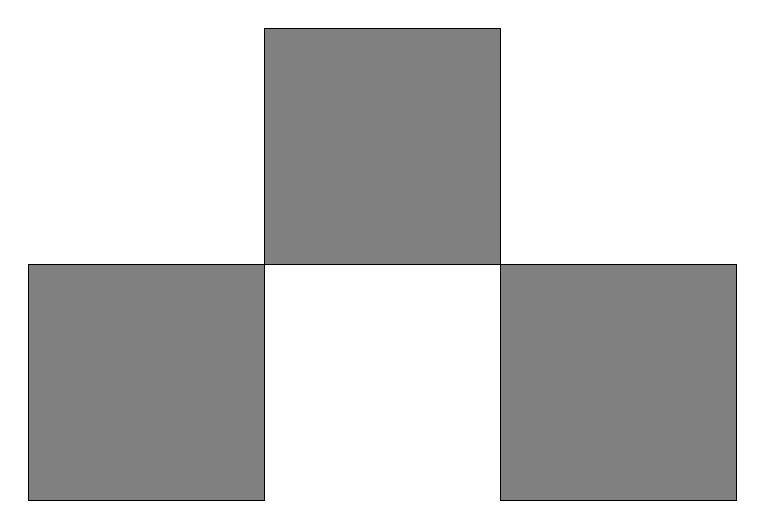
\begin{tikzpicture}%[line cap=round,line join=round,>=triangle 45,x=1.0cm,y=1.0cm]
\draw [fill=gray] (0,0) rectangle (3,3);
\draw [fill=gray] (3,3) rectangle (6,6);
\draw [fill=gray] (6,0) rectangle (9,3);
\end{tikzpicture}


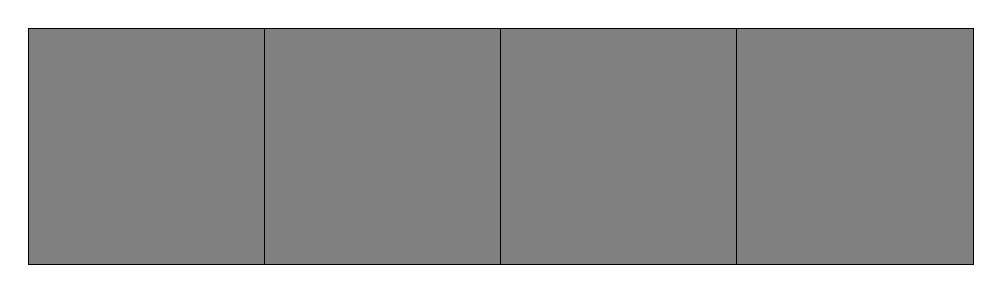
\begin{tikzpicture}%[line cap=round,line join=round,>=triangle 45,x=1.0cm,y=1.0cm]
\draw [fill=gray] (0,0) rectangle (3,3);
\draw [fill=gray] (3,0) rectangle (6,3);
\draw [fill=gray] (6,0) rectangle (9,3);
\draw [fill=gray] (9,0) rectangle (12,3);
\end{tikzpicture}

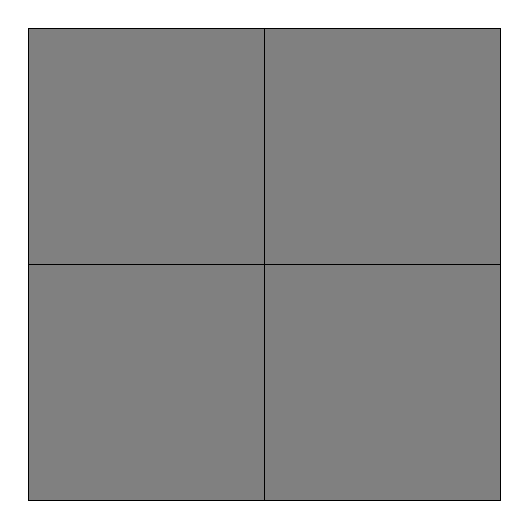
\begin{tikzpicture}%[line cap=round,line join=round,>=triangle 45,x=1.0cm,y=1.0cm]
\draw [fill=gray] (0,0) rectangle (3,3);
\draw [fill=gray] (0,3) rectangle (3,6);
\draw [fill=gray] (3,0) rectangle (6,3);
\draw [fill=gray] (3,3) rectangle (6,6);
\end{tikzpicture}


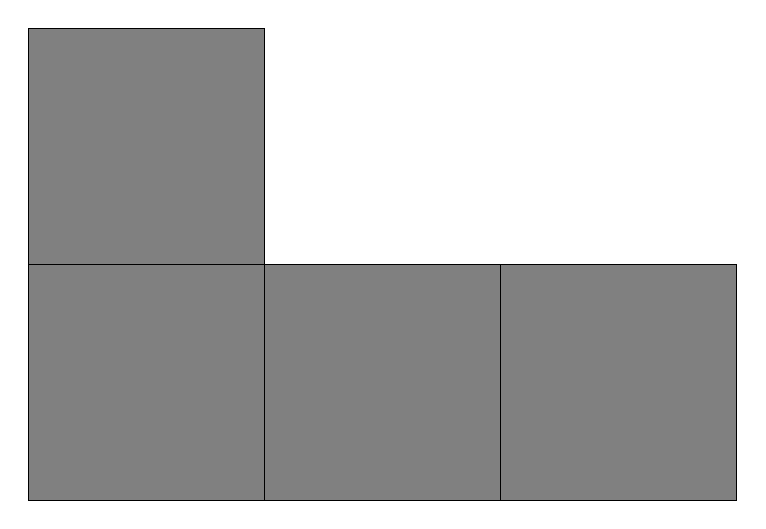
\begin{tikzpicture}%[line cap=round,line join=round,>=triangle 45,x=1.0cm,y=1.0cm]
\draw [fill=gray] (0,3) rectangle (3,6);
\draw [fill=gray] (0,0) rectangle (3,3);
\draw [fill=gray] (3,0) rectangle (6,3);
\draw [fill=gray] (6,0) rectangle (9,3);
\end{tikzpicture}

\begin{tikzpicture}%[line cap=round,line join=round,>=triangle 45,x=1.0cm,y=1.0cm]
\draw  (0,0) -- (3,3) -- (6,0);
\end{tikzpicture}


\begin{tikzpicture}%[line cap=round,line join=round,>=triangle 45,x=1.0cm,y=1.0cm]
\draw  (0,0) -- (3,3);
\draw  (2,0) -- (5,3);
\end{tikzpicture}


\begin{tikzpicture}%[line cap=round,line join=round,>=triangle 45,x=1.0cm,y=1.0cm]
\draw  (0,0) -- (3,3);
\draw  (3,0) -- (0,3);
\end{tikzpicture}

\begin{tikzpicture}%[line cap=round,line join=round,>=triangle 45,x=1.0cm,y=1.0cm]
\draw  (0,0) -- (3,3) -- (6,0) -- (9,3);
\end{tikzpicture}


\begin{tikzpicture}%[line cap=round,line join=round,>=triangle 45,x=1.0cm,y=1.0cm]
\draw  (0,0) -- (3,3);
\draw  (2,0) -- (5,3);
\draw  (4,0) -- (7,3);
\end{tikzpicture}

\begin{tikzpicture}%[line cap=round,line join=round,>=triangle 45,x=1.0cm,y=1.0cm]
\draw  (0,0) -- (3,3);
\draw  (4,0) -- (1,3);
\draw  (2,0) -- (5,3);
\end{tikzpicture}

\begin{tikzpicture}%[line cap=round,line join=round,>=triangle 45,x=1.0cm,y=1.0cm]
\draw  (0,0) -- (3,3) -- (0,6) -- (-3,3) -- (0,0);
\end{tikzpicture}

\begin{tikzpicture}%[line cap=round,line join=round,>=triangle 45,x=1.0cm,y=1.0cm]
\draw  (0,0) -- (3,3);
\draw  (2,0) -- (5,3);
\draw  (4,0) -- (7,3);
\draw  (6,0) -- (9,3);
\end{tikzpicture}

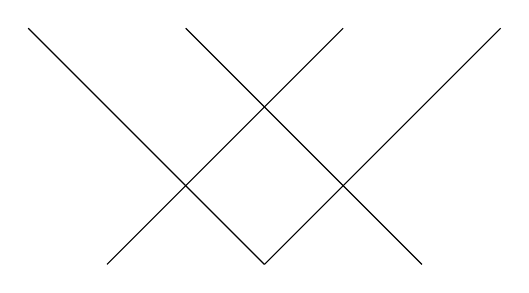
\begin{tikzpicture}%[line cap=round,line join=round,>=triangle 45,x=1.0cm,y=1.0cm]
\draw  (0,0) -- (3,3);
\draw  (4,0) -- (1,3);
\draw  (2,0) -- (5,3);
\draw (2,0) -- (-1,3);
\end{tikzpicture}

%triängulos
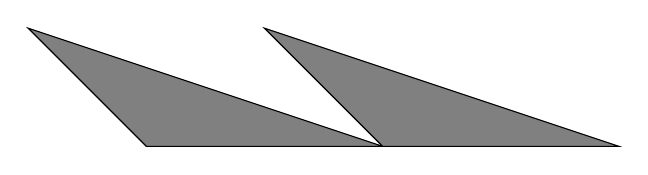
\begin{tikzpicture}%[line cap=round,line join=round,>=triangle 45,x=1.0cm,y=1.0cm]
\draw [fill=gray] (0,0) -- (3,0) -- (-1.5,1.5) -- cycle;
\draw [fill=gray] (3,0) -- (6,0) -- (1.5,1.5) -- cycle;
\end{tikzpicture}


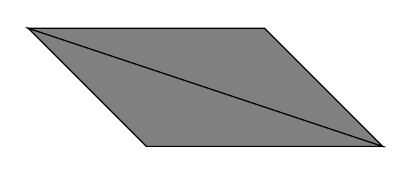
\begin{tikzpicture}%[line cap=round,line join=round,>=triangle 45,x=1.0cm,y=1.0cm]
\draw [fill=gray] (0,0) -- (3,0) -- (-1.5,1.5) -- cycle;
\draw [fill=gray] (3,0) -- (-1.5,1.5) -- (1.5,1.5) -- cycle;
\end{tikzpicture}

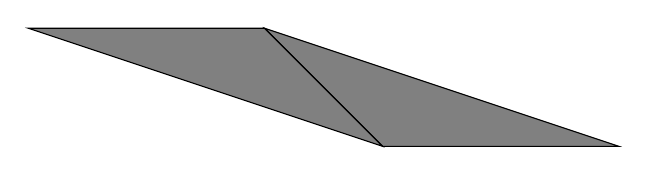
\begin{tikzpicture}%[line cap=round,line join=round,>=triangle 45,x=1.0cm,y=1.0cm]
\draw [fill=gray] (0,0) -- (3,0) -- (-1.5,1.5) -- cycle;
\draw [fill=gray] (0,0) -- (-1.5,1.5) -- (-4.5,1.5) -- cycle;
\end{tikzpicture}


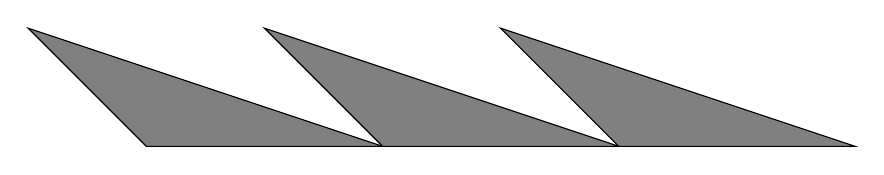
\begin{tikzpicture}%[line cap=round,line join=round,>=triangle 45,x=1.0cm,y=1.0cm]
\draw [fill=gray] (0,0) -- (3,0) -- (-1.5,1.5) -- cycle;
\draw [fill=gray] (3,0) -- (6,0) -- (1.5,1.5) -- cycle;
\draw [fill=gray] (6,0) -- (9,0) -- (4.5,1.5) -- cycle;
\end{tikzpicture}

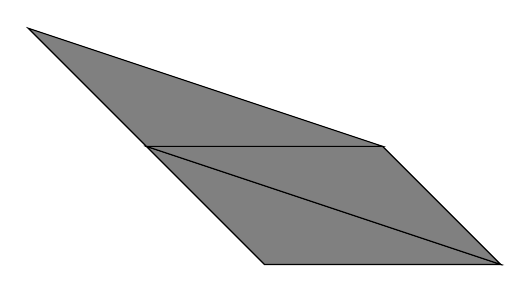
\begin{tikzpicture}%[line cap=round,line join=round,>=triangle 45,x=1.0cm,y=1.0cm]
\draw [fill=gray] (0,0) -- (3,0) -- (-1.5,1.5) -- cycle;
\draw [fill=gray] (3,0) -- (-1.5,1.5) -- (1.5,1.5) -- cycle;
\draw [fill=gray] (-1.5,1.5) -- (1.5,1.5) -- (-3,3) -- cycle;
%\draw [fill=gray] (1.5,1.5) -- (-3,3) -- (0,3) -- cycle;
\end{tikzpicture}

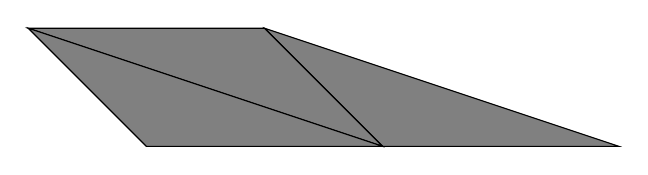
\begin{tikzpicture}%[line cap=round,line join=round,>=triangle 45,x=1.0cm,y=1.0cm]
\draw [fill=gray] (0,0) -- (3,0) -- (-1.5,1.5) -- cycle;
\draw [fill=gray] (0,0) -- (-1.5,1.5) -- (-4.5,1.5) -- cycle;
\draw [fill=gray] (-3,0) -- (0,0) -- (-4.5,1.5) -- cycle;
\end{tikzpicture}

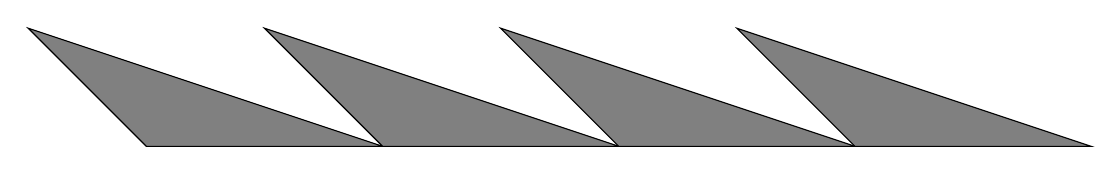
\begin{tikzpicture}%[line cap=round,line join=round,>=triangle 45,x=1.0cm,y=1.0cm]
\draw [fill=gray] (0,0) -- (3,0) -- (-1.5,1.5) -- cycle;
\draw [fill=gray] (3,0) -- (6,0) -- (1.5,1.5) -- cycle;
\draw [fill=gray] (6,0) -- (9,0) -- (4.5,1.5) -- cycle;
\draw [fill=gray] (9,0) -- (12,0) -- (7.5,1.5) -- cycle;
\end{tikzpicture}


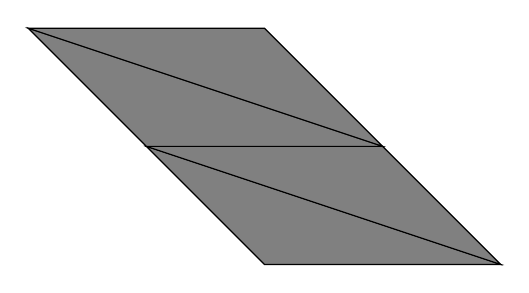
\begin{tikzpicture}%[line cap=round,line join=round,>=triangle 45,x=1.0cm,y=1.0cm]
\draw [fill=gray] (0,0) -- (3,0) -- (-1.5,1.5) -- cycle;
\draw [fill=gray] (3,0) -- (-1.5,1.5) -- (1.5,1.5) -- cycle;
\draw [fill=gray] (-1.5,1.5) -- (1.5,1.5) -- (-3,3) -- cycle;
\draw [fill=gray] (1.5,1.5) -- (-3,3) -- (0,3) -- cycle;
\end{tikzpicture}

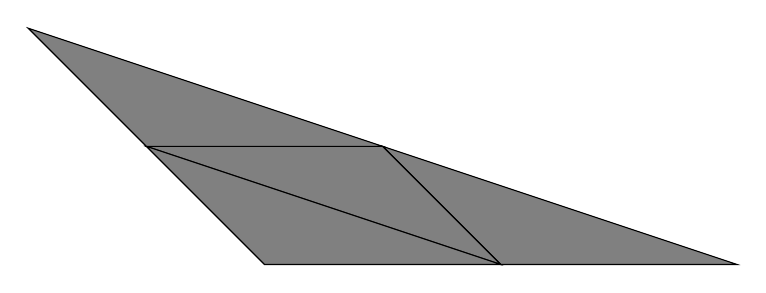
\begin{tikzpicture}%[line cap=round,line join=round,>=triangle 45,x=1.0cm,y=1.0cm]
\draw [fill=gray] (0,0) -- (3,0) -- (-1.5,1.5) -- cycle;
\draw [fill=gray] (0,0) -- (-1.5,1.5) -- (-4.5,1.5) -- cycle;
\draw [fill=gray] (-3,0) -- (0,0) -- (-4.5,1.5) -- cycle;
\draw [fill=gray] (-4.5,1.5) -- (-1.5,1.5) -- (-6,3) -- cycle;
\end{tikzpicture}

\end{document}
